\documentclass[a4j,dvipdfmx]{jarticle}
%\documentclass[uplatex,a4j,dvipdfmx]{ujarticle}
%\documentclass[uplatex,a4j,dvipdfmx]{jsarticle}
%\usepackage[uplatex,jis2004]{otf}
%----------------------------------------------------------------------
\usepackage{graphicx}
%\usepackage{amsmath}
%\usepackage{amssymb}
%\usepackage{bm}
%\usepackage{fancybox}
\usepackage{fancyhdr}
\usepackage{lastpage}
%\usepackage{color}
%\usepackage{multicol}
\usepackage{listings,jlisting}
\usepackage{ascmac}
\usepackage{url}
%----------------------------------------------------------------------
%\setlength{\topmargin}{-0.5in}
\setlength{\headheight}{15.0pt}
%%\setlength{\headsep}{0mm}
%\setlength{\oddsidemargin}{-0.5in}
%%\setlength{\evensidemargin}{-0.5in}
%\addtolength{\textwidth}{1.5in}
%\addtolength{\textheight}{1in}
%----------------------------------------------------------------------
%\setlength{\columnsep}{2zw}
%\setlength{\columnseprule}{0.4pt}
%----------------------------------------------------------------------
\pagestyle{fancy}
\lhead{2018/10/15}
\rhead{配布資料(\thepage / \pageref{LastPage})}
\cfoot{}
\chead{\textgt{オペレーティングシステム 第1回}}
%----------------------------------------------------------------------
\begin{document}
\def\lstlistingname{リスト}
\lstset{language=C,
  numbers=left,
  basicstyle={\small\ttfamily},
  columns=[l]{fullflexible},
  keepspaces=true,
  frame=shadowbox,
  commentstyle=\slshape
}
%----------------------------------------------------------------------

%\begin{figure}[hbtp]
%\begin{center}
%\includegraphics[height=2.5cm]{state.pdf}
%\caption{単語の長さをカウントするアルゴリズム}
%\end{center}
%\end{figure}

今回は、文字データの表現方法について学ぶ。

\begin{enumerate}

\item 原理

文字をコンピュータで表現するためには、
1年生で学んだASCIIコード表のような表を用いる。
ASCIIコード表は英字、数字、記号しか含んでいなかったので、
日本語や世界各国の文字を表すには不十分である。
そこで、ASCIIコード表の他に様々な文字コード表が用いられる。
次の手順で文字コード表を決める。

\begin{enumerate}
\item 扱う文字の範囲を決める

文字コード表に入れる文字の範囲を決める必要がある。
決めた範囲に含まれる文字の集合を{\bf 文字集合(character set)}と呼ぶ。

\item 文字に番号を付ける

文字集合に含まれる全ての文字に番号を付ける。
番号付けされた文字の集合を{\bf 符号化文字集合(coded character set)}と呼ぶ。

\item 番号をビット列に変換する方法を決める。

文字に付けた番号と実際のビット(バイト)列との変換方法を決める。
この変換方法のことを
{\bf 文字符号化方式(character encoding scheme)}と呼ぶ。
よく使う文字が短いビット列になるように符号化したりする。
複数の文字集合を同時に使用する時は、
どの文字集合に属するか分かるように符号化方式を決める。
\end{enumerate}

どのコンピュータでも同じ文字データが扱えるように、
符号化文字集合、文字符号化方式はISO\footnote{
ISO : International Organization for Standardization(国際標準化機構)
}、JIS\footnote{
JIS : Japan Industorial Standards(日本工業規格)
}等で規格化されている。
しかし、国により、コンピュータのOSにより、
アプリケーションプログラムにより、
採用している規格が完全に同じではないため、
どの規格か判定する際にミスがおこることがある。
{\bf 文字化け}は、判定ミスが起きた結果である。

Webブラウザが文字符号化方式の自動判定に成功した例と失敗した例を
図\ref{fig1}に示す。

\begin{figure}[hbtp]
\begin{center}
\begin{tabular}{c c}
\fbox{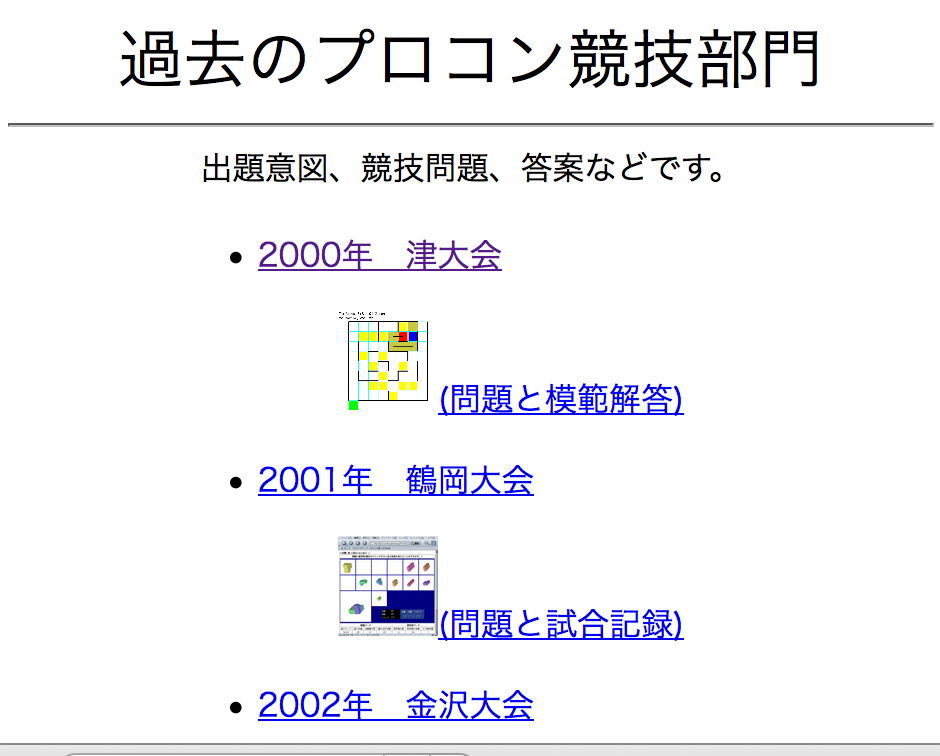
\includegraphics[scale=0.4]{screen1.png}} &
\fbox{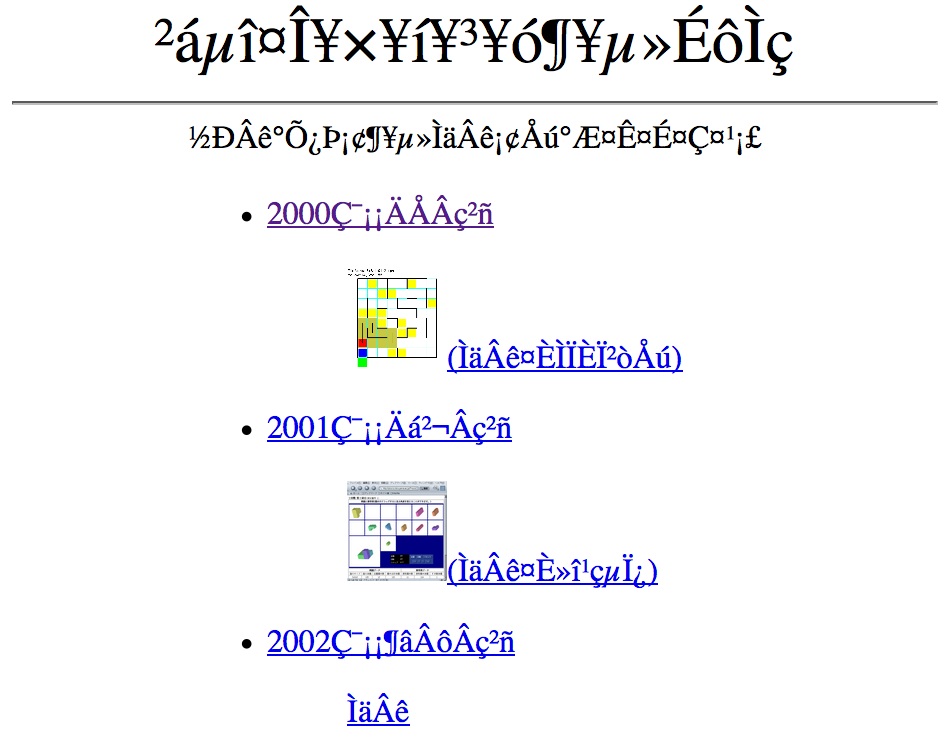
\includegraphics[scale=0.4]{screen2.png}} \\
(a) 正しく判定できた & (b) 正しく判定できなかった \\
\end{tabular}
\caption{文字化けの例}
\label{fig1}
\end{center}
\end{figure}

\newpage

\item 日本で使用される符号化文字集合

\begin{enumerate}
\item ASCII(American Standard Code for Infomation Interchange)文字コード表

図\ref{fig2}に示す符号化文字集合(coded character set)のこと。
1963年にアメリカ規格協会(ASCII)が定めた。
7ビットで、制御文字、記号、数字、英字大文字、英字小文字を表現できる。
制御文字と印刷可能文字あわせて128文字が含まれる。

\begin{figure}[hbtp]
\begin{center}
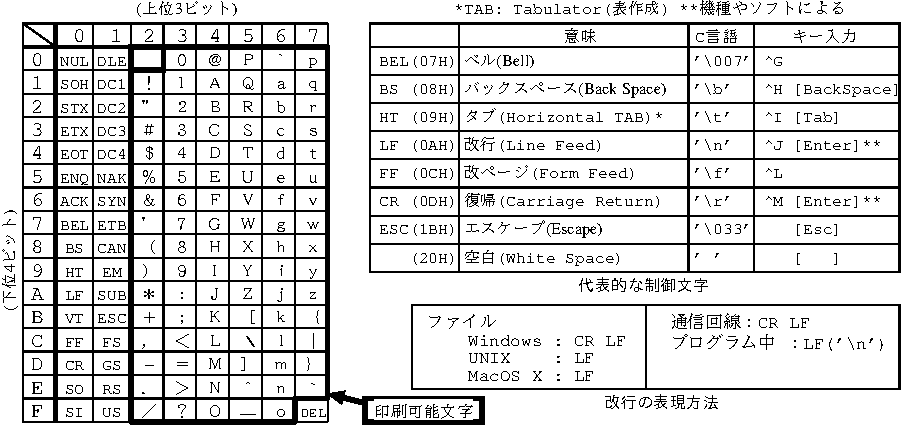
\includegraphics[scale=0.9]{ascii.pdf}
\caption{ASCII文字コード表}
\label{fig2}
\end{center}
\end{figure}

\item JIS X 0201(通称JIS 8ビットコード)

図\ref{fig3}に示す符号化文字集合のこと。
1969年に日本工業規格(JIS)に定められた。
8ビットで、制御文字、記号、数字、英字大文字、英字小文字、カタカナを表現できる。
制御文字と印刷可能文字あわせて191文字が含まれる。
制御文字、記号、数字、英字大文字、英字小文字の範囲は、
ASCIIと、ほぼ、同じになっている。

\begin{figure}[hbtp]
\begin{center}
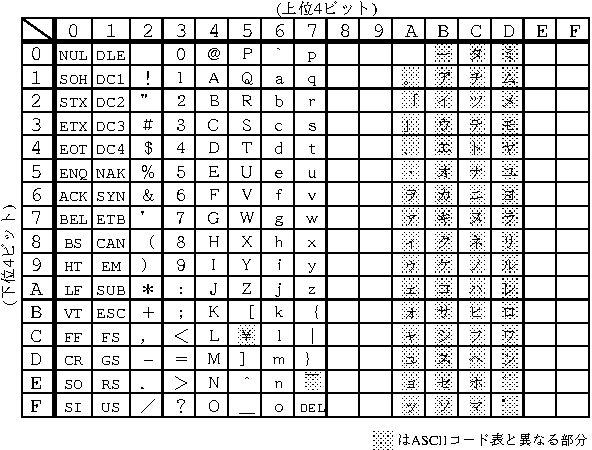
\includegraphics[scale=0.9]{jisx0201.pdf}
\caption{JIS 8ビット文字コード表}
\label{fig3}
\end{center}
\end{figure}

\newpage

\item JIS X 0208(通称JIS漢字)

図\ref{fig4}に示す符号化文字集合のこと。
1978年に日本工業規格(JIS)に定められた。
16ビットで、記号、英数字、かな、漢字などを表現できる。
{\bf 全角文字}6,879文字が登録されている。

\begin{figure}[hbtp]
\begin{center}
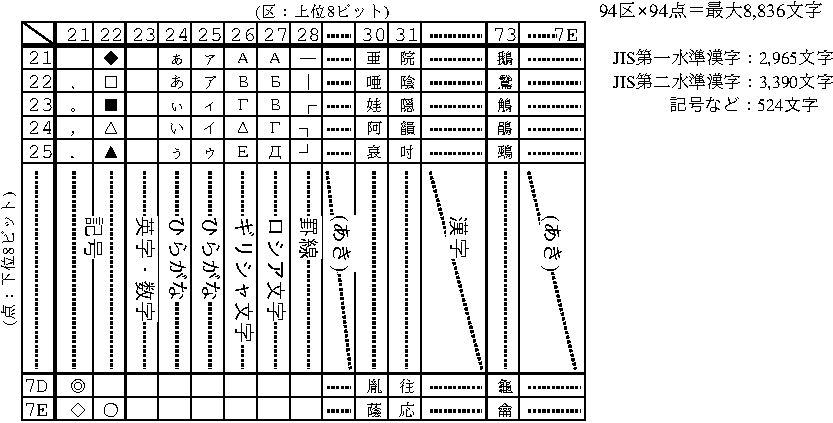
\includegraphics[scale=0.9]{jisx0208.pdf}
\caption{JIS漢字コード表}
\label{fig4}
\end{center}
\end{figure}

\item JIS X 0213(通称JIS拡張漢字)

図\ref{fig5}に示す符号化文字集合のこと。
2000年に日本工業規格(JIS)に定められた。
その後、2004年、2012年に改正されている。
コード表を2枚にすることで、より多くの文字を格納する。
{\bf 全角文字}11,223文字が登録されている。
JIS X 0208 を包含する上位規格(super set,上位集合)である。

\begin{figure}[hbtp]
\begin{center}
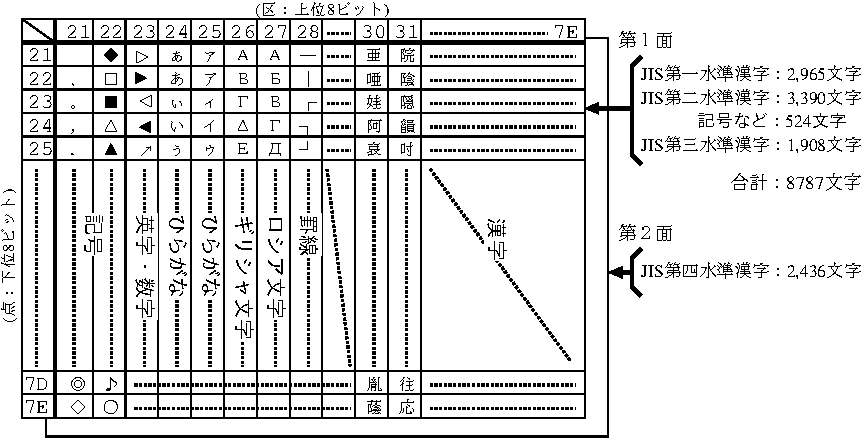
\includegraphics[scale=0.9]{jisx0213.pdf}
\caption{JIS拡張漢字コード表}
\label{fig5}
\end{center}
\end{figure}

\end{enumerate}

\newpage

\item 日本で使用される文字符号化方式(character encoding scheme)

文字データをファイルに格納したり通信路に送信したりするとき、
どんなバイト列に対応付けるか考える必要がある。

\begin{enumerate}
\item ISO-2022-JP(通称JISコード)

電子メール等で用いられることが多い。
エスケープシーケンスを用いて、
使用する符号化文字集合(文字コード表)を切換える(初期状態はASCII)。
7bitの範囲にエンコーディングされる。
次にエスケープシーケンスの一部を示す。

%\begin{table}
\begin{center}
{\tt
\begin{tabular}{l c l}
\fbox{ESC} \fbox{(}  \fbox{B}          & : & ASCII に切換える。 \\
\fbox{ESC} \fbox{(}  \fbox{J}          & : & JIS X 0201 の半角英数に切換える。 \\
\fbox{ESC} \fbox{\$} \fbox{B}          & : & JIS X 0208 に切換える。 \\
\fbox{ESC} \fbox{\$} \fbox{(} \fbox{Q} & : & JIS X 0213 の第1面に切換える。 \\
\fbox{ESC} \fbox{\$} \fbox{(} \fbox{P} & : & JIS X 0213 の第2面に切換える。 \\
%\multicolumn{3}
%{l}{以下は ISO/IEC 2022準拠のエスケープシーケンスでありISO-2022-JPの範囲外} \\
%\fbox{ESC} \fbox{(} \fbox{I}           & : & JIS X 0201 半角カナに切換える。 \\
\end{tabular}
}
%\caption{ISO-2022-JP で使用するエスケープシーケンス}
%\label{tab1}
\end{center}
%\end{table}

\hspace{-6mm}{\bf 例:}
``\verb/A亜a\¥/''をISO-2022-JPにエンコーディングした状態

{\hspace{-5mm}\small\tt\tabcolsep=0mm
\begin{tabular}{c ccc cc ccc cc ccc c ccc}
\fbox{41H}&                                % A
\fbox{1BH}&\fbox{24H}&\fbox{42H}&          % ESC $ B
\fbox{30H}&\fbox{21H}&                     % 亜
\fbox{1BH}&\fbox{28H}&\fbox{42H}&          % ESC ( B
\fbox{61H}&                                % a
\fbox{5CH}&                                % \
\fbox{1BH}&\fbox{28H}&\fbox{4AH}&          % ESC ( J
\fbox{5CH}&                                % ¥
\fbox{1BH}&\fbox{28H}&\fbox{42H}\\         % ESC ( B

'A'&                                       % A
ESC&'\$'&'B'&                              % ESC $ B
\multicolumn{2}{c}{'亜'} &                 % 亜
ESC&'('&'B'&                               % ESC ( B
'a'&                                       % a
'\verb/\/'&                                % \
ESC&'('&'J'&                               % ESC ( J
'¥'&                                       % ¥
ESC&'('&'B'\\                               % ESC ( B

&                                          % A
\multicolumn{3}{c}{<JIS X0208へ>}&         % ESC $ B
&&                                         % 亜
\multicolumn{3}{c}{<ASCIIへ>}&             % ESC ( B
&                                          % a
&                                          % \
\multicolumn{3}{c}{<JIS X0201へ>}&         % ESC ( J
&                                          % ¥
\multicolumn{3}{c}{<ASCIIへ>}              % ESC ( B
\\
\end{tabular}
}

\item EUC-JP(Extended UNIX Code for Japanese, 日本語EUC)

1980年代にUNIX上で日本語を扱うために考案された。
現在ではUTF-8が普及し使用されることが少なくなっている。
エスケープシーケンスを用いることなく、ASCIIとJIS X 0208を切換える。
符号化文字集合としてJIS X 0201を指定できないので、
半角の'¥'を表現することができない。
JIS X 0208 の文字はJIS漢字コードに 8080H を加えた値で表現する。

「ISO-2022-JPより短くエンコーディングできる」、
「変換規則が単純」、
「バイト列のどの部分が全角文字か直に分かる」、
「漢字を構成するバイトがASCIIと重ならない」等のメリットがある。

{\bf 例:} ``\verb/A亜a\\/''をEUC-JPにエンコーディングした状態

{\small\tt\tabcolsep=0mm
\begin{tabular}{ccc ccc}
\fbox{41H}&                                % A
\fbox{B0H}&\fbox{A1H}&                     % 亜
\fbox{61H}&                                % a
\fbox{5CH}&                                % \
\fbox{5CH}\\                               % \

'A'&                                       % A
\multicolumn{2}{c}{'亜'}&                  % 亜
'a'&                                       % a
'\verb/\/'&                                % \
'\verb/\/'\\                               % \
\end{tabular} 5CHは'\verb/\/'を表現する。
}

\item Shift\_JIS(Shift JIS code, SJIS)

1980年代にPCで日本語を扱うために考案され現在もWindowsで使用されている。
エスケープシーケンスを用いることなく、JIS X 0201とJIS X 0208を切換える。
符号化文字集合としてASCIIを指定できないので、
半角の'\verb/\/'を表現することができない\footnote{
日本のJava言語やC言語の教科書で'$\backslash${\tt n}'を
'¥n'と表記しているのはWindows使用前提だからか?
}。
JIS X 0208 の文字は、JIS漢字コードを
8140H - 9FFCH と E040H - FCFCH に変換して表現する。
計算で変換できるが若干複雑である。

「ISO-2022-JPより短くエンコーディングできる」、
「半角カナを1バイトで表現できる」等のメリットがある。

{\bf 例:} ``\verb/A亜a¥¥/''をShift\_JISにエンコーディングした状態

{\small\tt\tabcolsep=0mm
\begin{tabular}{ccc ccc}
\fbox{41H}&                                % A
\fbox{88H}&\fbox{9FH}&                     % 亜
\fbox{61H}&                                % a
\fbox{5CH}&                                % ¥
\fbox{5CH}\\                               % ¥

'A'&                                       % A
\multicolumn{2}{c}{'亜'}&                  % 亜
'a'&                                       % a
'¥'&                                       % ¥
'¥'\\                                      % ¥
\end{tabular} 5CHは'¥'を表現する。
}
\end{enumerate}

\newpage

\item Unicode(ユニコード)

符号化文字集合と文字符号化方式の両方を定めた文字コードの規格である。
単一(``Uni'')の巨大な文字コード表に、
世界中の全ての文字を収めようとしている。
符号化文字集合と文字符号化方式の両方を定めているので、
符号化に関する混乱も少ない。

当初、中国・日本・韓国の漢字を統一(CJK統合漢字)することで、
16bitで全ての文字にコードを割り振る計画だったが、
世界中の文字は予想以上に多かったため途中で21bitに変更された。
CJK統合漢字になっているのでJIS漢字コードとの変換には変換表が必要になる。

\begin{enumerate}
\item 歴史

1980年代後半から検討され1990年代前半に実用化された。
現在も世界各地の文字、古い文字(古代文字)、
新しい文字(絵文字)等が追加され続けている。

\begin{tabular}{l l l r l }
Unicode1.0.1 & 1992 & 16bit &  28,359文字 & JIS X 0201,0208,0212の文字収録 \\
Unicode2.0.0 & 1996 & 21bit &  38,950文字 & Unicode1.x.xとの互換性を失う   \\
Unicode3.0.0 & 2002 & 21bit &  95,221文字 & JIS X 0213へ対応               \\
Unicode4.0.0 & 2003 & 21bit &  96,447文字 & \\
Unicode5.0.0 & 2006 & 21bit &  99,089文字 & 楔文字や象形文字を追加\\
Unicode6.0.0 & 2012 & 21bit & 109,449文字 & 携帯絵文字追加 \\
Unicode7.0.0 & 2014 & 21bit & 113,021文字 & \\
Unicode8.0.0 & 2015 & 21bit & 120,737文字 & \\
Unicode9.0.0 & 2016 & 21bit & 128,172文字 & \\
Unicode10.0.0 & 2017 & 21bit & 136,690文字 & 変体仮名追加 \\
\end{tabular}

\item 符号化文字集合

図\ref{fig6}に示すように
Unicodeの文字コード表は17面(5bit)、256区(8bit)、256点(8bit)で構成される。
この表に最大111万文字を収容可能である。
半角ASCII文字から始まり、半角文字も全角文字もこの表に収録されている。

\begin{figure}[hbtp]
\begin{center}
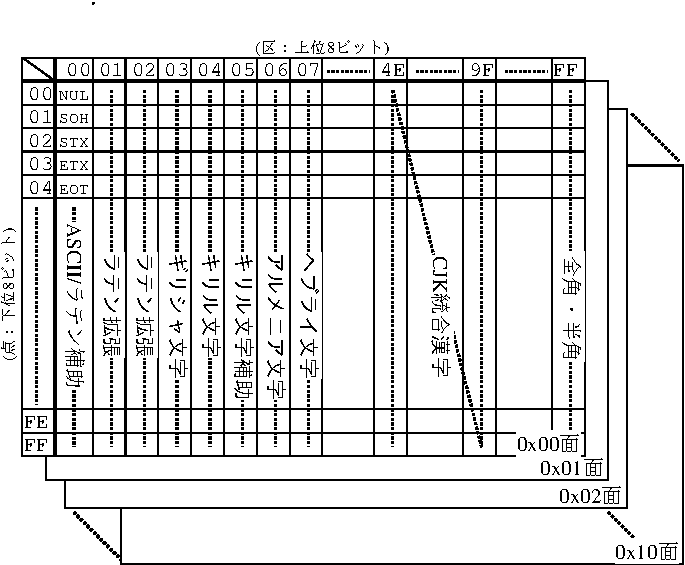
\includegraphics[scale=0.9]{unicode.pdf}
\caption{Unicode一覧}
\label{fig6}
\end{center}
\end{figure}

表の1文字を指定するためには、
21bit(5+8+8)のコード(Unicodeスカラ値)を用いる。
Unicodeスカラ値は、\verb/"U+1234"/のように
先頭に\verb/U+/を付加した16進数で表現する。

00面(U+0000〜U+FFFF)はBMP(Basic Multilingul Plane, 基本多言語面)と呼ばれる。
当初はBMPだけで全ての文字を格納する予定であった。
U+0000〜U+007FはASCIIコードと同じ配列になっている。
Java言語の\verb/char/型が16bitなのも、
16bitのUnicodeを格納することを前提に設計されたためである。

{\bf なお、完全なコード一覧は、
\url{https://ja.wikipedia.org/wiki/Unicode}
で見ることができる。}
面白い文字が見つかるので、一度、見てほしい。

\item 文字符号化方式

Unicode用の文字符号化方式(UTF:Unicode Transformation Format)が
定められている。
多くの方式が定められているが、代表的な方式は以下の3つである。

\begin{tabular}{l c l }
UTF-8  & : & 符号化結果は8bit,16bit,24bit,32bitのどれかになる。\\
       &   & 最もよく使用される方式である。半角英数字が小さく符号化できる。\\
UTF-16 & : & 00面を16bitに、その他は32bitに符号化する。\\
       &   & Unicodeが21bitになってから、Javaのchar型に使用されている。\\
UTF-32 & : & Unicodeの上位に0を付加し32bitに符号化する。\\
       &   & 固定長なので扱いやすい。\\
\end{tabular}

\item UTF-8による符号化手順

21bitのUnicodeのコードポイントを2進表記したものを、
表中のy、xに格納する。
yの部分には最低1つの1のビットがあるはずである。
符号化の結果は1〜4バイトになる。

{\tt%\small%\tabcolsep=1mm
\begin{tabular}{|l|cccc|c|}
\hline
\multicolumn{1}{|c}{Unicode} &
\multicolumn{4}{|c}{UTF-8(ビット列で表記)} &
\multicolumn{1}{|c|}{バイト数} \\
\hline
U+0000〜U+007F    & 0xxxxxxx &          &          &          & 1 \\
例 U+0000        & 00000000 & \multicolumn{3}{l|}{(00H)}     &   \\
例 U+007F        & 01111111 & \multicolumn{3}{l|}{(7FH)}     &   \\
\hline
U+0080〜U+07FF    & 110yyyyx & 10xxxxxx &          &          & 2 \\
例 U+0080        & 11000010 & 10000000 & \multicolumn{2}{l|}{(C2H 80H)} & \\
例 U+07FF        & 11011111 & 10111111 & \multicolumn{2}{l|}{(DFH BFH)} & \\
\hline
U+0800〜U+FFFF    & 1110yyyy & 10yxxxxx & 10xxxxxx &          & 3 \\
例 U+0800        & 11100000 & 10100000 & 10000000 &          &   \\
                  & (E0H)    & (A0H)    & (80H)    &          &   \\
例 U+FFFF        & 11101111 & 10111111 & 10111111 &          &   \\
                  & (EFH)    & (BFH)    & (BFH)    &          &   \\
\hline
U+10000〜U+1FFFFF & 11110yyy & 10yyxxxx & 10xxxxxx & 10xxxxxx & 4 \\
例 U+10000       & 11110000 & 10010000 & 10000000 & 10000000 &   \\
                 & (F0H)    & (90H)    & (80H)    & (80H)    &   \\
例 U+1FFFFF      & 11110111 & 10111111 & 10111111 & 10111111 &   \\
                  & (F7H)    & (BFH)    & (BFH)    & (BFH)    &   \\
\hline
\end{tabular}}

\end{enumerate}

\newpage

\item 文字コード変換コマンド(iconv)

UNIXやMacでは、iconv\footnote{
International Codeset Conversion Library に付属する
文字コード変換プログラムである。
}%コマンドや、nkf\footnote{Network Kanji Filter}
コマンドを
使用して文字符号化方式(文字コード)を変換することができる。
次に、iconvコマンドの使い方を簡単に説明する。

\begin{lstlisting}[numbers=none]
書式1: iconv [-f ENCODE] [-t ENCODE] [テキストファイル ...]

書式2: iconv -l

説明: ENCODE は文字符号化方式を表す文字列である。

       書式1の場合、-f ENCODE で指定される符号化方式のデータを入力し、
       -t ENCODE で指定される符号化方式に変換し、標準出力に出力する。
       テキストファイルが指定されない場合は標準入力からデータを入力する。

       書式2は、iconvが扱うことができる文字符号化方式の一覧を表示する。

実行例:
$ emacs utf8.txt                                   # 何かテキストファイルを作る
$ iconv -f UTF-8 -t ISO-2022-JP utf8.txt > iso.txt # ISO-2022-JPに変換する
\end{lstlisting}

\item 16進ダンプコマンド(hexdump)

hexdumpコマンドはファイルか標準入力のバイト列を16進数に変換して表示する。
次に簡単な説明と実行例を示す。

\begin{lstlisting}[numbers=none]
書式: hexdump [オプション] [ファイル ...]

説明: hexdump は、ファイルの内容を16進数に変換して標準出力に出力する。
       [ファイル ...] が省略された場合はファイルの代わりに標準入力を使用する。

実行例:
$ cat ascii.txt 
ABCDEFG
$ hexdump ascii.txt 
0000000 41 42 43 44 45 46 47 0a                        
0000008
$ iconv -f UTF-8 -t UTF-32BE ascii.txt  | hexdump
0000000 00 00 00 41 00 00 00 42 00 00 00 43 00 00 00 44
0000010 00 00 00 45 00 00 00 46 00 00 00 47 00 00 00 0a
0000020
$ iconv -f UTF-8 -t UTF-32LE ascii.txt  | hexdump 
0000000 41 00 00 00 42 00 00 00 43 00 00 00 44 00 00 00
0000010 45 00 00 00 46 00 00 00 47 00 00 00 0a 00 00 00
0000020
$

# UTF-32BE : ビッグエンディアン(上位桁からのバイト順)
# UTF-32LE : リトルエンディアン(下位桁からのバイト順)
\end{lstlisting}

\newpage

\item 宿題

半角英数字、
%半角カナ、
全角カナ、全角漢字、半角バックスラッシュ(ASCII)、
半角円記号(JIS X 0201)等、色々な文字を含むテキストファイルを観察する。

\begin{enumerate}
\item ファイルの作成

%残念ながら日頃使用している emacs は、
%円記号を入力できない\footnote{
%C言語やJava言語を入力するとき、
%バックスラッシュ、円記号の間違えをおこさないように、
%IE電算のMacのemacsでは円マークが入力できないようにカスタマイズしてある。
%}ので、
%半角カナが表示できないかも知れない\footnote{
%動作確認していない。
%}等の問題がある。
%Mac標準の「テキストエディット」、または、「vi(vim)」を使用して
%色々な文字を含むテキストファイルを作成する。
%テキストエディット([ランチャー]→[その他]→[テキストエディット])では、
%[¥]で'¥'が、[Option]+[¥]で'$\backslash$'が入力できる。

IE電算のMacのemacsでは、[¥]キーでバックスラッシュが入力される。
[command]+[¥]で'$\backslash$'が入力できる。

\begin{lstlisting}[numbers=none]
$ cat x0208UTF8.txt
0Aa!
あア亜院
a\¥A
$
\end{lstlisting}

\item 様々な文字符号化方式に変換し結果を16進数ダンプして確認する。

\begin{lstlisting}[numbers=none]
$ iconv -f UTF-8 -t UTF-32BE x0208UTF8.txt | hexdump
0000000 00 00 00 30 00 00 00 41 00 00 00 61 00 00 00 21
0000010 00 00 00 0a 00 00 30 42 00 00 30 a2 00 00 4e 9c
0000020 00 00 96 62 00 00 00 0a 00 00 00 61 00 00 00 5c
0000030 00 00 00 a5 00 00 00 41 00 00 00 0a            
000003c
$
\end{lstlisting}

\item 16進数ダンプの内容を解析する。

\begin{lstlisting}[numbers=none]
// UTF-32 に変換した結果(Unicodeのコードポイントと対応がわかりやすい)
00 00 00 30 : 0  (U+0030) : BMP(ASCII領域)
00 00 00 41 : A  (U+0041) : BMP(ASCII領域)
00 00 00 61 : a  (U+0061) : BMP(ASCII領域)
00 00 00 21 : !  (U+0021) : BMP(ASCII領域)
00 00 00 0a : LF (U+000a) : BMP(ASCII領域)
00 00 30 42 : あ (U+3042) : BMP(かな領域)
00 00 30 a2 : ア (U+30a2) : BMP(かな領域)
00 00 4e 9c : 亜 (U+4e9c) : BMP(CJK統合漢字領域)
00 00 96 62 : 院(U+9662) : BMP(CJK統合漢字領域)
00 00 00 0a : LF (U+000a) : BMP(ASCII領域)
00 00 00 61 : a  (U+0061) : BMP(ASCII領域)
00 00 00 5c : \  (U+005c) : BMP(ASCII領域)
00 00 00 a5 : ¥  (U+00a5) : BMP(全角・半角領域)
00 00 00 41 : A  (U+0041) : BMP(ASCII領域)
00 00 00 0a : LF (U+000a) : BMP(ASCII領域)
\end{lstlisting}

\item 上記の変換と解析を幾つかの文字符号化方式について確認する。
(UTF-8、ISO-2022-JP、SJIS、 EUC-JP、...)

\item EUC-JP に変換した後 UTF-8 に戻すとどうなるか確認する。

\begin{lstlisting}[numbers=none]
$ iconv -f UTF-8 -t EUC-JP x0208UTF8.txt | iconv -f EUC-JP -t UTF-8 | hexdump
$ iconv -f UTF-8 -t EUC-JP x0208UTF8.txt | iconv -f EUC-JP -t UTF-8
\end{lstlisting}

\end{enumerate}

%\lstinputlisting[numbers=none]{example.txt}

\end{enumerate}
\end{document}
